\documentclass[11pt,a4paper]{article}
\usepackage[utf8]{inputenc}
\usepackage[T1]{fontenc}
\usepackage[magyar]{babel}
\usepackage{lmodern}
\usepackage[margin=2.2cm]{geometry}
\usepackage{graphicx}
\usepackage{longtable,booktabs,array,calc}
\usepackage{xcolor}
\usepackage{listings}
\usepackage[hidelinks]{hyperref}
\usepackage{fancyvrb}
\usepackage{amsmath}
\usepackage{textcomp}
\DeclareUnicodeCharacter{2212}{\ensuremath{-}}
\DeclareUnicodeCharacter{2192}{\ensuremath{\rightarrow}}
\DeclareUnicodeCharacter{03A3}{\ensuremath{\Sigma}}
\DeclareUnicodeCharacter{00B7}{\ensuremath{\cdot}}
\DeclareUnicodeCharacter{00D7}{\ensuremath{\times}}
\DeclareUnicodeCharacter{2550}{=}
\DeclareUnicodeCharacter{2500}{-}
\DeclareUnicodeCharacter{2551}{|}
\DeclareUnicodeCharacter{2502}{|}
\DeclareUnicodeCharacter{2566}{+}

\graphicspath{{../}}
\newcommand{\rootdir}{../../..}

% pandoc által használt makrók
\newcommand{\passthrough}[1]{#1}
\providecommand{\tightlist}{\setlength{\itemsep}{0pt}\setlength{\parskip}{0pt}}
\def\LTcaptype{none}
\newcounter{none}

\definecolor{kodhatter}{RGB}{248,248,248}
\definecolor{kulcsszo}{RGB}{0,0,160}
\definecolor{komment}{RGB}{0,120,0}
\definecolor{sztring}{RGB}{160,40,40}
\lstset{
  basicstyle=\ttfamily\footnotesize,
  backgroundcolor=\color{kodhatter},
  keywordstyle=\color{kulcsszo}\bfseries,
  commentstyle=\color{komment}\itshape,
  stringstyle=\color{sztring},
  numbers=left, numberstyle=\tiny\color{gray}, numbersep=6pt,
  breaklines=true, breakatwhitespace=false, columns=fullflexible, keepspaces=true,
  showstringspaces=false, frame=single, rulecolor=\color{gray!40},
  tabsize=4, extendedchars=true, upquote=true,
  literate=
    {á}{{\'a}}1 {é}{{\'e}}1 {í}{{\'i}}1 {ó}{{\'o}}1 {ú}{{\'u}}1
    {Á}{{\'A}}1 {É}{{\'E}}1 {Í}{{\'I}}1 {Ó}{{\'O}}1 {Ú}{{\'U}}1
    {ö}{{\"o}}1 {ü}{{\"u}}1 {ő}{{\H{o}}}1 {ű}{{\H{u}}}1
    {Ö}{{\"O}}1 {Ü}{{\"U}}1 {Ő}{{\H{O}}}1 {Ű}{{\H{U}}}1
    {→}{{$\rightarrow$}}1 {←}{{$\leftarrow$}}1 {–}{{--}}1 {—}{{---}}1
    {·}{{$\cdot$}}1 {×}{{$\times$}}1 {±}{{$\pm$}}1 {≥}{{$\geq$}}1 {≤}{{$\leq$}}1
    {Σ}{{$\Sigma$}}1 {−}{{-}}1 {…}{{...}}1 {„}{{,,}}1 {”}{{''}}1
    {═}{{=}}1 {╦}{{+}}1 {║}{{|}}1 {─}{{-}}1 {│}{{|}}1 {┌}{{+}}1 {┐}{{+}}1 {└}{{+}}1 {┘}{{+}}1
}

\title{\texttt{sumo\_morl}\\[4pt]\large Többcélú megerősítéses tanulás jelzőlámpa-vezérléshez SUMO-ban}
\date{}

\begin{document}
\maketitle
\tableofcontents
\newpage

% Automatikusan generálva a docs/sumo_morl/*.md fájlokból (build_latex.py)
\hypertarget{sumo_morl--tuxf6bbcuxe9luxfa-megerux151suxedtuxe9ses-tanuluxe1s-jelzux151luxe1mpa-vezuxe9rluxe9shez}{%
\section{sumo\_morl -- többcélú
megerősítéses tanulás
jelzőlámpa-vezérléshez}\label{sumo_morl--tuxf6bbcuxe9luxfa-megerux151suxedtuxe9ses-tanuluxe1s-jelzux151luxe1mpa-vezuxe9rluxe9shez}}

A \passthrough{\lstinline!sumo\_morl!}
egy oktatási célú Python könyvtár,
amellyel \textbf{forgalomtechnikai
előismeretek nélkül} lehet többcélú
megerősítéses tanulással (MORL)
jelzőlámpa-vezérlő ágenseket fejleszteni
a \href{https://eclipse.dev/sumo/}{SUMO}
forgalomszimulátorban.

Minden forgalomtechnikai rész készen
van:

\begin{itemize}
\tightlist
\item
  egy \textbf{T-csomópont} hálózata (a
  keleti ág ketté van osztva balra
  kanyarodó és egyenes sávra),
\item
  a \textbf{közbenső idők} (intergreen)
  a repó közbensőidő-számító kódjával
  készülnek, a csomópont geometriájából,
\item
  a \textbf{fázisok}, és köztük a
  szabályos \textbf{átmenetek} (sárga,
  piros, piros-sárga),
\item
  \textbf{indukcióshurok-detektorok}
  minden bejövő sávon,
\item
  \textbf{forgalmi igény} generálása
  (epizódonként véletlen),
\item
  klasszikus \textbf{összehasonlító
  vezérlők} (fix idejű, járműkövető,
  mohó).
\end{itemize}

A hallgató feladata „csak'' az ágens:
minden döntési pontban meg kell
mondania, \textbf{melyik fázis} legyen a
következő.

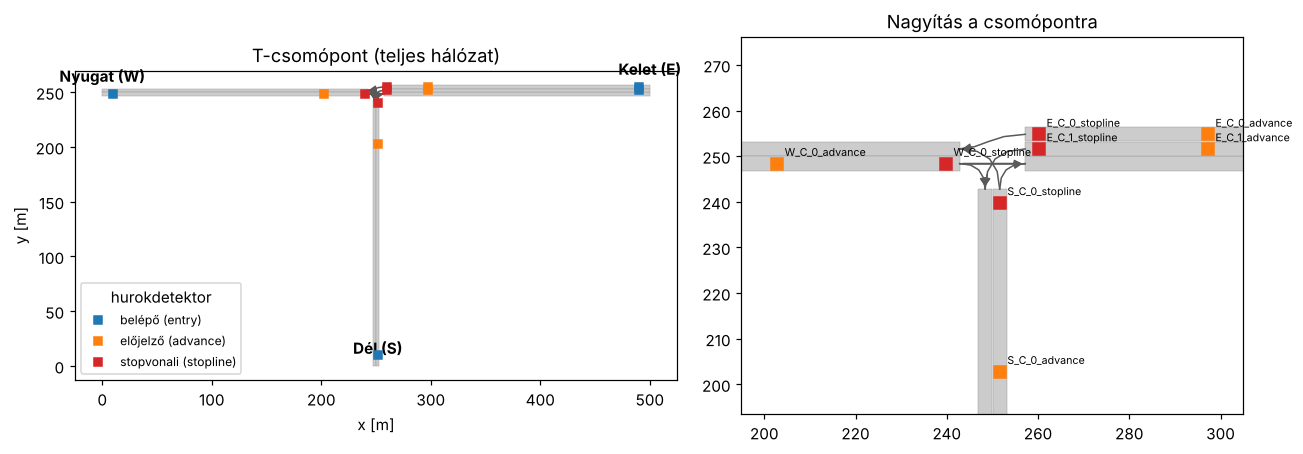
\includegraphics[width=\linewidth]{img/csomopont.png}

\hypertarget{telepuxedtuxe9s}{%
\subsection{Telepítés}\label{telepuxedtuxe9s}}

Python 3.9 vagy újabb kell. A repó
gyökeréből:

\begin{lstlisting}[language=bash]
python -m venv .venv
source .venv/bin/activate          # Windows: .venv\Scripts\activate
pip install -e .                   # a könyvtár + SUMO (eclipse-sumo pip csomag)
pip install -e ".[rl]"             # + Stable-Baselines3 (a 03-as példához)
\end{lstlisting}

A SUMO-t az
\passthrough{\lstinline!eclipse-sumo!}
pip csomag telepíti, így külön
SUMO-telepítés nem kell. Ha már van SUMO
a gépen és a
\passthrough{\lstinline!SUMO\_HOME!}
környezeti változó be van állítva, azt
használja a könyvtár.

Ellenőrzés:

\begin{lstlisting}[language=bash]
python -m pytest                                   # a könyvtár tesztjei (kb. fél perc)
python examples/sumo_morl/00_demo_fix_ido.py --gui # demó: fix idejű program a SUMO felületén
\end{lstlisting}

\hypertarget{demuxf3-fix-idejux171-program}{%
\subsection{Demó: fix idejű
program}\label{demuxf3-fix-idejux171-program}}

Mielőtt bármilyen ágenst írnál, nézd meg
a működést a legegyszerűbb, klasszikus
vezérléssel: a fázisok mindig ugyanabban
a sorrendben, mindig ugyanannyi ideig
kapnak zöldet (alapértelmezés: 30, 10 és
15 s).

\begin{lstlisting}[language=bash]
python examples/sumo_morl/00_demo_fix_ido.py --gui                # SUMO grafikus felülettel
python examples/sumo_morl/00_demo_fix_ido.py --green 40 10 20     # más zöldidők
\end{lstlisting}

A program kiírja a fázisokat, az
átmeneteket és a ciklusidőt, majd minden
fázisváltásnál a detektorokból becsült
járműszámot. A végén megadja a
jutalmakat és a valós mutatókat, és
elmenti az első két ciklus jelzéstervét
(\passthrough{\lstinline!fix\_ido\_jelzesterv.png!}):

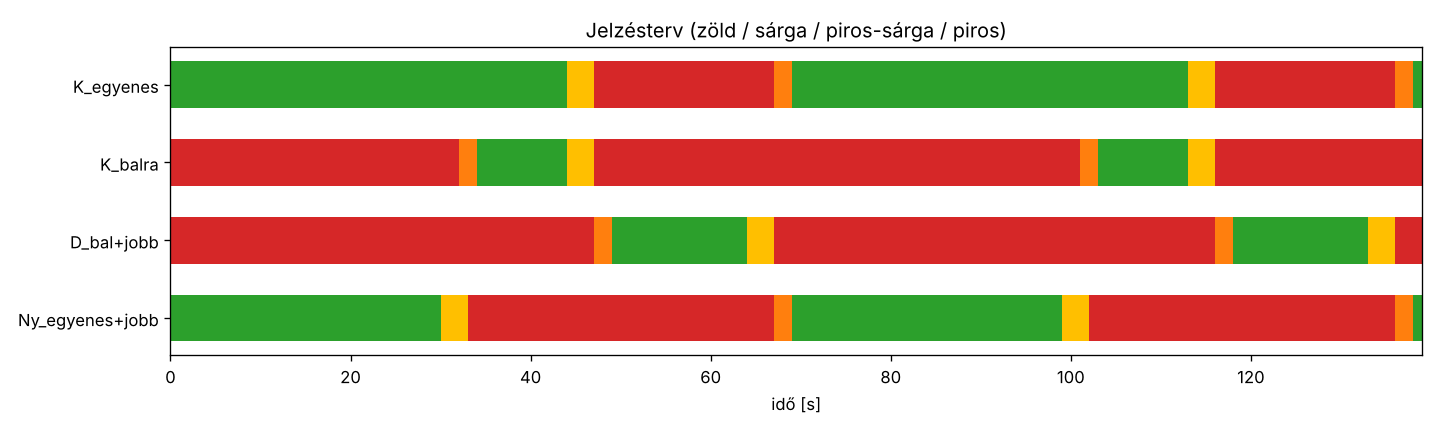
\includegraphics[width=\linewidth]{img/fix_ido_jelzesterv.png}

\hypertarget{gyors-kezduxe9s}{%
\subsection{Gyors
kezdés}\label{gyors-kezduxe9s}}

\begin{lstlisting}[language=Python]
import numpy as np
from sumo_morl import TJunctionMOEnv

env = TJunctionMOEnv(objectives=("queue", "fairness", "switches"), episode_length=3600)
obs, info = env.reset(seed=0)

done = False
total = np.zeros(env.reward_dim)
while not done:
    action = env.action_space.sample()       # <- ide jön az ágensed
    obs, reward, terminated, truncated, info = env.step(action)
    total += reward                          # a reward egy VEKTOR (célonként egy elem)
    done = terminated or truncated

print(dict(zip(env.objective_names, total)))
env.close()
\end{lstlisting}

\begin{itemize}
\tightlist
\item
  \passthrough{\lstinline!action!}: a
  következő fázis sorszáma (0, 1 vagy
  2).
\item
  \passthrough{\lstinline!obs!}: 55
  elemű vektor {[}0, 1{]} tartományban,
  csak detektoradatokból és a vezérlő
  saját állapotából.
\item
  \passthrough{\lstinline!reward!}:
  \passthrough{\lstinline!numpy!}
  vektor, a kiválasztott célfüggvények
  sorrendjében.
\item
  \passthrough{\lstinline!info!}:
  részletes adatok (aktuális fázis,
  nyers detektoradatok, és --
  \textbf{csak kiértékeléshez} --
  SUMO-ból kiolvasott valós mutatók).
\end{itemize}

Egycélú RL könyvtárral (pl.
Stable-Baselines3) a jutalmat
skalarizálni kell:

\begin{lstlisting}[language=Python]
from stable_baselines3 import DQN
from sumo_morl import TJunctionMOEnv, LinearScalarization

env = LinearScalarization(TJunctionMOEnv(), weights=[0.6, 0.3, 0.1])
model = DQN("MlpPolicy", env).learn(50_000)
\end{lstlisting}

A grafikus felülethez add meg a
\passthrough{\lstinline!gui=True!}
paramétert: ekkor a
\passthrough{\lstinline!sumo-gui!} indul
el, és látható, mit csinál az ágens.

\hypertarget{puxe9lduxe1k}{%
\subsection{Példák}\label{puxe9lduxe1k}}

\begin{longtable}[]{@{}>{\raggedright\arraybackslash}p{0.32\linewidth}>{\raggedright\arraybackslash}p{0.64\linewidth}@{}}
\toprule\noalign{}
Fájl & Mit mutat be \\
\midrule\noalign{}
\endhead
\bottomrule\noalign{}
\endlastfoot
\passthrough{\lstinline!examples/sumo\_morl/00\_demo\_fix\_ido.py!}
& \textbf{demó:} klasszikus fix idejű
program, konzolos eseménynapló,
jelzésterv-ábra
(\passthrough{\lstinline!--gui!}-val
látható a szimuláció) \\
\passthrough{\lstinline!examples/sumo\_morl/01\_ismerkedes.py!}
& a környezet, a jelzésterv kiírása,
véletlen ágens \\
\passthrough{\lstinline!examples/sumo\_morl/02\_baseline\_osszehasonlitas.py!}
& klasszikus vezérlők azonos forgalmon,
Pareto-ábra \\
\passthrough{\lstinline!examples/sumo\_morl/03\_sb3\_sulyozott\_tanitas.py!}
& DQN tanítása több súlyvektorral,
Pareto-front, hipertérfogat \\
\passthrough{\lstinline!examples/sumo\_morl/04\_sajat\_celfuggveny.py!}
& saját célfüggvény definiálása \\
\end{longtable}

\hypertarget{a-kuxf6nyvtuxe1r-feluxe9puxedtuxe9se}{%
\subsection{A könyvtár
felépítése}\label{a-kuxf6nyvtuxe1r-feluxe9puxedtuxe9se}}

\begin{longtable}[]{@{}>{\raggedright\arraybackslash}p{0.36\linewidth}>{\raggedright\arraybackslash}p{0.60\linewidth}@{}}
\toprule\noalign{}
Modul & Tartalom \\
\midrule\noalign{}
\endhead
\bottomrule\noalign{}
\endlastfoot
\passthrough{\lstinline!sumo\_morl/env.py!}
&
\passthrough{\lstinline!TJunctionMOEnv!}
-- a Gymnasium környezet \\
\passthrough{\lstinline!sumo\_morl/objectives.py!}
& célfüggvények (jutalomkomponensek),
\passthrough{\lstinline!register\_objective!} \\
\passthrough{\lstinline!sumo\_morl/detectors.py!}
& hurokdetektorok elhelyezése, olvasása,
aggregálása \\
\passthrough{\lstinline!sumo\_morl/intergreen.py!}
& jelzőcsoportok, fázisok, átmenetek a
közbensőidő-számításból \\
\passthrough{\lstinline!sumo\_morl/scenario.py!}
& a T-csomópont forgatókönyv (hálózat +
jelzésterv + detektorok) \\
\passthrough{\lstinline!sumo\_morl/network.py!}
& a hálózat generálása
\passthrough{\lstinline!netconvert!}-tel \\
\passthrough{\lstinline!sumo\_morl/traffic.py!}
& forgalmi igény
(\passthrough{\lstinline!Demand!}) és
route fájl \\
\passthrough{\lstinline!sumo\_morl/policies.py!}
& összehasonlító vezérlők \\
\passthrough{\lstinline!sumo\_morl/morl.py!}
& skalarizálás, súlyok, Pareto-front,
hipertérfogat, kiértékelés \\
\passthrough{\lstinline!sumo\_morl/visualize.py!}
& ábrák (csomópont, fázisok, közbenső
idők, epizód) \\
\passthrough{\lstinline!sumo\_morl/data/t\_junction.net.xml!}
& a kész hálózat \\
\end{longtable}

A közbenső időket a repó gyökerében
lévő, már meglévő
\passthrough{\lstinline!geometry\_utils.py!}
és
\passthrough{\lstinline!sumo\_parser.py!}
számolja (ugyanaz a kód, amit a GUI-s
közbensőidő-számító is használ); a
\passthrough{\lstinline!pip install -e .!}
ezeket is telepíti.


\hypertarget{a-csomuxf3pont-a-fuxe1zisok-uxe9s-a-kuxf6zbensux151-idux151k}{%
\section{A csomópont, a fázisok és a
közbenső
idők}\label{a-csomuxf3pont-a-fuxe1zisok-uxe9s-a-kuxf6zbensux151-idux151k}}

\begin{quote}
Röviden: \textbf{ezzel nem kell
foglalkoznod.} Az ágens csak egy fázis
sorszámát választja; a környezet
gondoskodik róla, hogy a jelzőlámpák
mindig szabályosan és biztonságosan
váltsanak. Ez az oldal azért van, hogy
értsd, mi történik a háttérben.
\end{quote}

\hypertarget{a-csomuxf3pont}{%
\subsection{A
csomópont}\label{a-csomuxf3pont}}

Egyszerű T-csomópont, jobbkezes
forgalommal. Minden ág 250 m hosszú, a
megengedett sebesség 50 km/h.

\begin{lstlisting}
        Nyugat (W) ═══════════════╦═══════════════ Kelet (E)
                                  ║
                                  ║
                               Dél (S)
\end{lstlisting}

\begin{longtable}[]{@{}lll@{}}
\toprule\noalign{}
Ág & Bejövő sáv & Mozgások \\
\midrule\noalign{}
\endhead
\bottomrule\noalign{}
\endlastfoot
Nyugat (W) &
\passthrough{\lstinline!W\_C\_0!} &
egyenesen keletre + jobbra délre (közös
sáv) \\
Kelet (E) &
\passthrough{\lstinline!E\_C\_0!} &
egyenesen nyugatra \\
Kelet (E) &
\passthrough{\lstinline!E\_C\_1!} &
balra, délre (külön kanyarodósáv) \\
Dél (S) &
\passthrough{\lstinline!S\_C\_0!} &
balra nyugatra + jobbra keletre (közös
sáv) \\
\end{longtable}

A keleti („jobb oldali'') bejövő ág
tehát \textbf{ketté van osztva}: a balra
kanyarodók külön sávban várakoznak, így
nem tartják fel az egyenesen haladókat.

\hypertarget{fogalmak}{%
\subsection{Fogalmak}\label{fogalmak}}

\begin{itemize}
\tightlist
\item
  \textbf{Jelzőcsoport}: azon mozgások
  halmaza, amelyek mindig ugyanazt a
  jelzést kapják. Nálunk egy bejövő sáv
  = egy jelzőcsoport (4 csoport).
\item
  \textbf{Konfliktus}: két csoport
  konfliktusos, ha a járműveik útvonala
  keresztezi egymást vagy összefut.
  Konfliktusos csoportok nem kaphatnak
  egyszerre zöldet.
\item
  \textbf{Fázis}: konfliktusmentes
  csoportok halmaza, amelyek egyszerre
  kapnak zöldet.
\item
  \textbf{Közbenső idő} (intergreen)
  \passthrough{\lstinline!k(i→j)!}: az
  \passthrough{\lstinline!i!} csoport
  zöldjének vége és a vele konfliktusos
  \passthrough{\lstinline!j!} csoport
  zöldjének kezdete között minimálisan
  eltelő idő. Ennyi idő kell ahhoz, hogy
  az utolsó, még zölden behajtó jármű
  elhagyja az ütközési pontot, mielőtt
  az új irány járművei odaérnek.
\item
  \textbf{Átmenet}: két fázis közötti
  jelzésképsorozat (sárga, piros,
  piros-sárga).
\end{itemize}

\hypertarget{a-kuxf6zbensux151-idux151k-szuxe1muxedtuxe1sa}{%
\subsection{A közbenső idők
számítása}\label{a-kuxf6zbensux151-idux151k-szuxe1muxedtuxe1sa}}

A közbenső időket a repó meglévő
közbensőidő-számító kódja
(\passthrough{\lstinline!geometry\_utils.py!},
\passthrough{\lstinline!sumo\_parser.py!})
számolja a SUMO hálózat geometriájából:

\begin{enumerate}
\def\labelenumi{\arabic{enumi}.}
\tightlist
\item
  minden mozgás pályáját simított
  görbével közelíti, és kiszámolja a
  kanyarodási sugarat, abból a
  sebességet,
\item
  megkeresi a pályák ütközési pontjait,
\item
  kiszámolja a kiürítési és a behaladási
  időt:
  \passthrough{\lstinline!k = 3 s + (kiürítési út + 6 m) / v\_kiürítő − behaladási út / v\_belépő!},
  felfelé kerekítve.
\end{enumerate}

A
\passthrough{\lstinline!sumo\_morl.intergreen!}
modul ebből a mozgásszintű mátrixból
jelzőcsoport-szintű mátrixot képez (a
csoport mozgásainak maximuma):

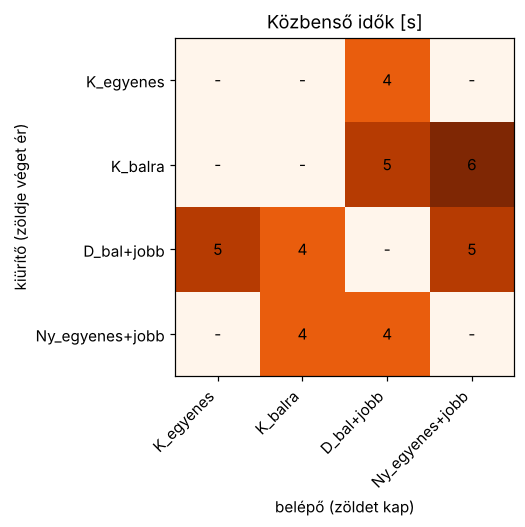
\includegraphics[width=0.5\linewidth]{img/kozbenso_idok.png}

\hypertarget{a-fuxe1zisok}{%
\subsection{A
fázisok}\label{a-fuxe1zisok}}

A fázisokat a konfliktusmátrixból
kapjuk: a konfliktusmentes csoportok
maximális halmazai (gráfelméletben:
klikkek). Ebből a csomópontból pontosan
három adódik:

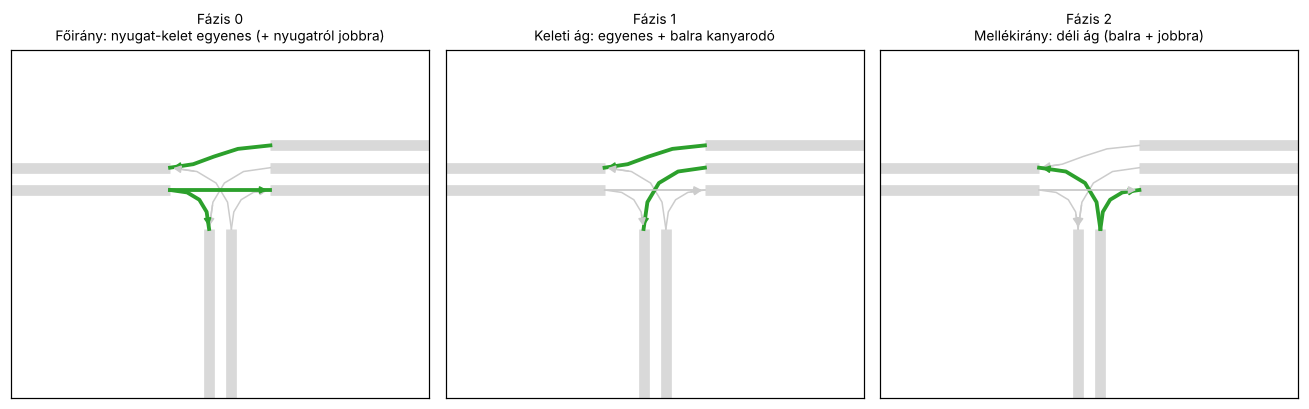
\includegraphics[width=\linewidth]{img/fazisok.png}

\begin{longtable}[]{@{}ll>{\raggedright\arraybackslash}p{0.69\linewidth}@{}}
\toprule\noalign{}
Fázis & Zöldet kap & Megjegyzés \\
\midrule\noalign{}
\endhead
\bottomrule\noalign{}
\endlastfoot
0 & \passthrough{\lstinline!W\_C\_0!} +
\passthrough{\lstinline!E\_C\_0!} &
főirány mindkét irányban egyenesen (+
nyugatról jobbra) \\
1 & \passthrough{\lstinline!E\_C\_0!} +
\passthrough{\lstinline!E\_C\_1!} &
keleti ág: egyenes + védett balra
kanyarodás \\
2 & \passthrough{\lstinline!S\_C\_0!} &
déli mellékág \\
\end{longtable}

\hypertarget{az-uxe1tmenetek}{%
\subsection{Az
átmenetek}\label{az-uxe1tmenetek}}

Fázisváltáskor a környezet automatikusan
lejátssza az átmenetet:

\begin{itemize}
\tightlist
\item
  a megszűnő csoportok 3 s
  \textbf{sárgát}, majd pirosat kapnak,
\item
  az induló csoportok annyi idő után
  kapnak zöldet, amennyit a közbenső idő
  előír (legalább 2 s), és előtte 2 s
  \textbf{piros-sárgát} kapnak,
\item
  a mindkét fázisban zöld csoportok
  végig zöldek maradnak.
\end{itemize}

Az átmenetek hossza (s):

\begin{longtable}[]{@{}llll@{}}
\toprule\noalign{}
honnan \textbackslash{} hova & 0 & 1 &
2 \\
\midrule\noalign{}
\endhead
\bottomrule\noalign{}
\endlastfoot
\textbf{0} & -- & 4 & 4 \\
\textbf{1} & 6 & -- & 5 \\
\textbf{2} & 5 & 5 & -- \\
\end{longtable}

Az átmenetek alatt (és utána a minimális
zöldidő alatt) az ágens nem dönt; ez a
forgalomtechnikában \textbf{elveszett
idő}, ezért a túl gyakori váltás rontja
az áteresztőképességet.

\hypertarget{kiuxedruxe1s-uxe9s-uxe1bruxe1k-a-sajuxe1t-guxe9peden}{%
\subsection{Kiírás és ábrák a saját
gépeden}\label{kiuxedruxe1s-uxe9s-uxe1bruxe1k-a-sajuxe1t-guxe9peden}}

\begin{lstlisting}[language=Python]
from sumo_morl import TJunctionScenario
from sumo_morl.visualize import plot_scenario, plot_phases, plot_intergreen

sc = TJunctionScenario()
print(sc.describe())                 # csoportok, közbenső idők, fázisok, átmenetek, detektorok
plot_scenario(sc).savefig("csomopont.png")
plot_phases(sc).savefig("fazisok.png")
\end{lstlisting}

A hálózat újragenerálása (pl. más
ághosszal) csak haladóknak kell:
\passthrough{\lstinline!python -m sumo\_morl.network!},
illetve
\passthrough{\lstinline!sumo\_morl.network.build\_network()!}.


\hypertarget{megfigyeluxe9s-hurokdetektorok-csak-muxe9rhetux151-adatok}{%
\section{Megfigyelés: hurokdetektorok
(csak mérhető
adatok)}\label{megfigyeluxe9s-hurokdetektorok-csak-muxe9rhetux151-adatok}}

Egy valódi csomópontban a vezérlő
\textbf{nem látja} a járműveket: nem
tudja, hány autó áll a sorban, ki mióta
vár, vagy hová tart. Amit tud, azt az
úttestbe épített
\textbf{indukcióshurok-detektorok}
mérik. Hogy az ágens a valóságba is
átvihető legyen, a
\passthrough{\lstinline!sumo\_morl!}
megfigyelése és jutalma
\textbf{kizárólag} ilyen adatokból
készül.

\hypertarget{a-detektorok-elhelyezuxe9se}{%
\subsection{A detektorok
elhelyezése}\label{a-detektorok-elhelyezuxe9se}}

Minden bejövő sávon (4 sáv) három hurok
van, összesen 12:

\begin{lstlisting}
 ág eleje                                                    stopvonal
 |--[entry]--------------------------------[advance]---------[stopline]|
    10 m az ág elejétől                     40 m-re a          3 m-re a
                                            stopvonaltól       stopvonaltól
\end{lstlisting}

\begin{longtable}[]{@{}>{\raggedright\arraybackslash}p{0.24\linewidth}>{\raggedright\arraybackslash}p{0.72\linewidth}@{}}
\toprule\noalign{}
Típus & Mire jó \\
\midrule\noalign{}
\endhead
\bottomrule\noalign{}
\endlastfoot
\passthrough{\lstinline!entry!} (belépő)
& a csomópont felé érkező járművek
számlálása \\
\passthrough{\lstinline!advance!}
(előjelző) & közeledő járművek
érzékelése; ha tartósan foglalt, a sor
már idáig ér \\
\passthrough{\lstinline!stopline!}
(stopvonali) & a stopvonalon áthaladó
járművek számlálása, a sor eleje \\
\end{longtable}

A detektorok azonosítója
\passthrough{\lstinline!<sáv>\_<típus>!},
pl.
\passthrough{\lstinline!E\_C\_1\_stopline!}.

\hypertarget{mit-muxe9r-egy-hurok}{%
\subsection{Mit mér egy
hurok?}\label{mit-muxe9r-egy-hurok}}

\begin{longtable}[]{@{}l>{\raggedright\arraybackslash}p{0.54\linewidth}>{\raggedright\arraybackslash}p{0.31\linewidth}@{}}
\toprule\noalign{}
Mennyiség & Jelentés & Valóságban \\
\midrule\noalign{}
\endhead
\bottomrule\noalign{}
\endlastfoot
\passthrough{\lstinline!count!} & a
lépés alatt áthaladt járművek száma &
impulzusszámlálás \\
\passthrough{\lstinline!occupancy!} & az
idő hányadában volt jármű a hurok felett
(0..1) & foglaltság \\
\passthrough{\lstinline!speed!} &
átlagsebesség a hurkon (m/s), jármű
nélkül a megengedett sebesség & dupla
hurokkal mérhető \\
\passthrough{\lstinline!gap!} & a
legutóbbi érzékelés óta eltelt idő (s) &
időrés, a járműkövető vezérlők alapja \\
\end{longtable}

\hypertarget{becsuxfclt-juxe1rmux171szuxe1m-uxe1gankkuxe9nt-bemenetkimenet-muxf3dszer}{%
\subsubsection{Becsült járműszám
ágankként (bemenet--kimenet
módszer)}\label{becsuxfclt-juxe1rmux171szuxe1m-uxe1gankkuxe9nt-bemenetkimenet-muxf3dszer}}

Az \passthrough{\lstinline!entry!} és a
\passthrough{\lstinline!stopline!}
hurkok számlálóiból folyamatosan
számoljuk, hány jármű van a két hurok
között:
\passthrough{\lstinline!N(t) = N(t−1) + belépők − kilépők!}.
Ez a klasszikus, gyakorlatban is
használt sorhossz-becslés. Tesztjeink
szerint a becslés legfeljebb 1--3
járművel tér el a SUMO-beli valós
értéktől.

\hypertarget{a-megfigyeluxe9svektor}{%
\subsection{A
megfigyelésvektor}\label{a-megfigyeluxe9svektor}}

A \passthrough{\lstinline!obs!} egy 55
elemű, \passthrough{\lstinline![0, 1]!}
tartományba normalizált
\passthrough{\lstinline!float32!}
vektor:

\begin{longtable}[]{@{}>{\raggedright\arraybackslash}p{0.35\linewidth}l>{\raggedright\arraybackslash}p{0.50\linewidth}@{}}
\toprule\noalign{}
Elemek & Darab & Normalizálás \\
\midrule\noalign{}
\endhead
\bottomrule\noalign{}
\endlastfoot
minden detektorra:
\passthrough{\lstinline!count!},
\passthrough{\lstinline!occupancy!},
\passthrough{\lstinline!speed!},
\passthrough{\lstinline!gap!} & 12 × 4 =
48 & forgalom / 1800 jármű/óra;
foglaltság; sebesség / sebességkorlát;
időrés / 60 s \\
ágankénti becsült járműszám (W, E, S) &
3 & / az ág tárolókapacitása
(\textasciitilde7 m / jármű) \\
aktuális fázis (one-hot) & 3 & 0 vagy
1 \\
az aktuális zöld eddigi hossza & 1 & /
120 s \\
\end{longtable}

Az elemek neveit az
\passthrough{\lstinline!env.observation\_names()!}
adja vissza, pl.
\passthrough{\lstinline!'E\_C\_1\_stopline.occupancy'!},
\passthrough{\lstinline!'approach\_S.vehicles'!},
\passthrough{\lstinline!'phase\_2'!}.

Ha saját megfigyelést szeretnél (pl.
csak a stopvonali hurkokat), írj egy
\passthrough{\lstinline!gymnasium.ObservationWrapper!}-t,
és használd az
\passthrough{\lstinline!info["detectors"]!}
nyers adatait:

\begin{lstlisting}[language=Python]
import gymnasium as gym
import numpy as np

class OnlyStopline(gym.ObservationWrapper):
    def __init__(self, env):
        super().__init__(env)
        self.idx = [i for i, n in enumerate(env.unwrapped.observation_names())
                    if "stopline" in n or n.startswith("phase_")]
        self.observation_space = gym.spaces.Box(0, 1, (len(self.idx),), np.float32)

    def observation(self, obs):
        return obs[self.idx]
\end{lstlisting}

\hypertarget{a-nyers-detektoradatok-infodetectors}{%
\subsection{\texorpdfstring{A nyers
detektoradatok:
\texttt{info{[}"detectors"{]}}}{A nyers detektoradatok: info{[}"detectors"{]}}}\label{a-nyers-detektoradatok-infodetectors}}

Egy
\passthrough{\lstinline!DetectorSnapshot!}
objektum az utolsó lépés aggregált
adataival:

\begin{lstlisting}[language=Python]
snap = info["detectors"]
snap.duration                         # a lépés hossza [s]
snap.count, snap.occupancy, snap.speed, snap.gap   # numpy tömbök, detektoronként
snap.approach_vehicles                # {'W': 12.0, 'E': 4.0, 'S': 7.0} – becslés a lépés végén
snap.approach_vehicle_seconds         # ugyanez a lépés másodperceire összegezve
snap.select(kind="stopline")          # bool maszk a szűréshez
snap.select(lane_id="E_C_1")
snap.by_id()["E_C_1_stopline"]        # {'count': 2.0, 'occupancy': 0.31, ...}
\end{lstlisting}

\hypertarget{amit-szuxe1nduxe9kosan-nem-kap-meg-az-uxe1gens}{%
\subsection{Amit szándékosan NEM kap meg
az
ágens}\label{amit-szuxe1nduxe9kosan-nem-kap-meg-az-uxe1gens}}

\begin{itemize}
\tightlist
\item
  jármű-azonosítók, pozíciók, úticélok,
\item
  pontos sorhossz és várakozási idő,
\item
  emisszió, utazási idő.
\end{itemize}

Ezeket a környezet
\passthrough{\lstinline!ground\_truth=True!}
(alapértelmezett) beállítással az
\passthrough{\lstinline!info["ground\_truth"]!}
alatt kiírja, de \textbf{csak
kiértékeléshez} (pl. a dolgozatban annak
bemutatására, hogy a tanult vezérlő
tényleg csökkenti-e a késést). A
megfigyelésbe vagy a jutalomba beépíteni
„csalás'', mert a valóságban nem
elérhető.

\begin{longtable}[]{@{}>{\raggedright\arraybackslash}p{0.30\linewidth}>{\raggedright\arraybackslash}p{0.66\linewidth}@{}}
\toprule\noalign{}
\passthrough{\lstinline!info["ground\_truth"]!}
kulcs & Jelentés \\
\midrule\noalign{}
\endhead
\bottomrule\noalign{}
\endlastfoot
\passthrough{\lstinline!halting\_vehicle\_seconds!}
& álló járművek száma másodpercenként
összegezve (a bejövő ágakon) \\
\passthrough{\lstinline!mean\_delay\_per\_vehicle!}
& ugyanez elosztva az elindult járművek
számával {[}s{]} \\
\passthrough{\lstinline!mean\_travel\_time!}
& a célba ért járművek átlagos utazási
ideje {[}s{]} \\
\passthrough{\lstinline!co2\_g!} &
CO2-kibocsátás a bejövő ágakon
{[}g{]} \\
\passthrough{\lstinline!departed!},
\passthrough{\lstinline!arrived!} &
elindult / célba ért járművek \\
\passthrough{\lstinline!waiting\_to\_enter!}
& a hálózatba be sem tudó
(visszatorlódott) járművek \\
\end{longtable}


\hypertarget{jutalomvektor-cuxe9lfuxfcggvuxe9nyek}{%
\section{Jutalomvektor:
célfüggvények}\label{jutalomvektor-cuxe9lfuxfcggvuxe9nyek}}

A többcélú tanulásban a jutalom nem egy
szám, hanem egy \textbf{vektor}: minden
elem egy-egy célt mér. A célok általában
ellentmondanak egymásnak (pl. kevés
várakozás vs. kevés fázisváltás), ezért
nincs egyetlen „legjobb'' vezérlés,
hanem \textbf{Pareto-optimális}
vezérlések halmaza van.

A célokat a környezet létrehozásakor
választod ki, a jutalomvektor ebben a
sorrendben tartalmazza őket:

\begin{lstlisting}[language=Python]
env = TJunctionMOEnv(objectives=("queue", "fairness", "switches"))   # alapértelmezés
env.objective_names    # ('queue', 'fairness', 'switches')
\end{lstlisting}

\hypertarget{beuxe9puxedtett-cuxe9lfuxfcggvuxe9nyek}{%
\subsection{Beépített
célfüggvények}\label{beuxe9puxedtett-cuxe9lfuxfcggvuxe9nyek}}

Konvenció: \textbf{nagyobb = jobb} (a
költségek negatív előjelűek). Minden
érték a lépés másodperceire összegzett
mennyiség, így az epizód összjutalma a
teljes időre vett integrál, függetlenül
attól, hogy a lépések milyen hosszúak. A
\passthrough{\lstinline!skála!} csak
arra szolgál, hogy a tipikus értékek 1
körüliek legyenek.

\begin{longtable}[]{@{}l>{\raggedright\arraybackslash}p{0.27\linewidth}l>{\raggedright\arraybackslash}p{0.42\linewidth}@{}}
\toprule\noalign{}
Név & Képlet (lépésenként) & Skála & Mit
jelent \\
\midrule\noalign{}
\endhead
\bottomrule\noalign{}
\endlastfoot
\passthrough{\lstinline!queue!} &
−Σ\_ágak Σ\_másodpercek becsült
járműszám & 0,01 & a teljes késleltetés
közelítése (kevés jármű a csomópont
előtt) \\
\passthrough{\lstinline!fairness!} &
−max\_ág Σ\_másodpercek becsült
járműszám & 0,02 & méltányosság: a
legrosszabb helyzetű ág se várjon
sokat \\
\passthrough{\lstinline!switches!} & −1,
ha volt fázisváltás & 1 & stabil
vezérlés, kevés elveszett idő az
átmenetekben \\
\passthrough{\lstinline!throughput!} & a
stopvonali hurkokon áthaladt járművek &
0,1 & áteresztőképesség (főleg
túltelített helyzetben számít) \\
\passthrough{\lstinline!stopline\_occupancy!}
& −Σ stopvonali foglalt másodpercek &
0,1 & a stopvonalnál álló járművek
közelítése \\
\end{longtable}

Mindegyik csak hurokdetektor-adatokból
(és a vezérlő saját állapotából) számol.
A listát a programból is lekérheted:

\begin{lstlisting}[language=Python]
from sumo_morl import list_objectives
print(list_objectives())
\end{lstlisting}

\hypertarget{sajuxe1t-cuxe9lfuxfcggvuxe9ny}{%
\subsection{Saját
célfüggvény}\label{sajuxe1t-cuxe9lfuxfcggvuxe9ny}}

Egy célfüggvény egy függvény
\passthrough{\lstinline!(snap, ctx) -> float!},
ahol

\begin{itemize}
\tightlist
\item
  \passthrough{\lstinline!snap!} a lépés
  hurokadatai
  (\passthrough{\lstinline!DetectorSnapshot!},
  lásd Megfigyelés),
\item
  \passthrough{\lstinline!ctx!} egy
  szótár:
  \passthrough{\lstinline!phase\_changed!},
  \passthrough{\lstinline!phase!},
  \passthrough{\lstinline!duration!},
  \passthrough{\lstinline!time!},
  \passthrough{\lstinline!forced!}.
\end{itemize}

\begin{lstlisting}[language=Python]
from sumo_morl import TJunctionMOEnv, register_objective

@register_objective("side_road_queue", scale=0.02,
                    doc="A déli mellékág becsült járműszáma (min.)")
def side_road_queue(snap, ctx):
    return -snap.approach_vehicle_seconds["S"]

env = TJunctionMOEnv(objectives=("queue", "side_road_queue"))
\end{lstlisting}

Fontos: a célfüggvényben \textbf{ne}
kérdezd le a SUMO-t közvetlenül (TraCI),
mert akkor valóságban nem mérhető adatot
használnál.

\hypertarget{skalarizuxe1luxe1s}{%
\subsection{Skalarizálás}\label{skalarizuxe1luxe1s}}

A legtöbb RL algoritmus skalár jutalmat
vár. A két legegyszerűbb módszer:

\begin{itemize}
\tightlist
\item
  \textbf{Lineáris skalarizálás}
  (\passthrough{\lstinline!LinearScalarization!}
  wrapper):
  \passthrough{\lstinline!r = w · r\_vec!},
  rögzített súlyvektorral. Különböző
  súlyokkal külön ágenseket tanítva
  feltérképezhető a Pareto-front (konvex
  része).
\item
  \textbf{Súly-kondicionált ágens}
  (\passthrough{\lstinline!WeightConditioned!}
  wrapper): epizódonként véletlen súlyt
  sorsol, és azt a megfigyelés végére
  fűzi. Egyetlen háló tanulja meg az
  összes kompromisszumot; kiértékeléskor
  a kívánt súlyt kell megadni.
\end{itemize}

Mindkettő az eredeti vektort az
\passthrough{\lstinline!info["vector\_reward"]!}
alatt is visszaadja.

Fejlettebb MORL módszerek (pl. Pareto
Q-learning, Envelope Q-learning,
nemlineáris hasznossági függvények) a
vektor-jutalommal közvetlenül
megvalósíthatók.


\hypertarget{a-kuxf6rnyezet-api-ja}{%
\section{A környezet
API-ja}\label{a-kuxf6rnyezet-api-ja}}

\begin{lstlisting}[language=Python]
from sumo_morl import TJunctionMOEnv, Demand

env = TJunctionMOEnv(
    objectives=("queue", "fairness", "switches"),  # jutalomkomponensek
    demand=None,              # None = epizódonként véletlen igény
    episode_length=3600,      # szimulált másodperc
    decision_interval=5,      # "maradok" akció: ennyi másodperccel hosszabb zöld
    min_green=5,              # váltás után ennyi ideig biztosan zöld
    max_green=None,           # pl. 90: ennél hosszabb zöld után kényszerített váltás
    warmup=0,                 # ennyi s fix idejű bemelegítés az epizód elején
    gui=False,                # sumo-gui megjelenítés
    seed=None,
    ground_truth=True,        # info["ground_truth"] kiértékeléshez
    record_signals=False,     # env.signal_log: másodpercenkénti jelzéskép (jelzésterv-ábrához)
)
\end{lstlisting}

A környezet a
\href{https://gymnasium.farama.org/}{Gymnasium}
API-t és az MO-Gymnasium konvenciót
követi (vektor jutalom +
\passthrough{\lstinline!env.reward\_space!}).
\passthrough{\lstinline!gym.make("sumo\_morl/TJunction-v0", ...)!}
is működik.

\hypertarget{akciuxf3}{%
\subsection{Akció}\label{akciuxf3}}

\passthrough{\lstinline!env.action\_space = Discrete(3)!}:
a \textbf{következő fázis} sorszáma.

\begin{itemize}
\tightlist
\item
  Ha az akció az aktuális fázis → a zöld
  \passthrough{\lstinline!decision\_interval!}
  (5) másodperccel meghosszabbodik.
\item
  Ha más fázis → lefut a szabályos
  átmenet (4--6 s, lásd jelzésterv),
  majd az új fázis
  \passthrough{\lstinline!min\_green!}
  (5) másodpercig biztosan zöld. Csak
  ezután jön a következő döntés.
\end{itemize}

Emiatt a lépések hossza \textbf{változó}
(5 s vagy 9--11 s). Az
\passthrough{\lstinline!info["elapsed"]!}
megadja az adott lépés hosszát. A
jutalmak a lépés másodperceire
összegzettek, így ez nem torzítja az
összjutalmat. (Ha diszkontálsz, érdemes
lehet a diszkontot a lépés hosszához
igazítani:
\passthrough{\lstinline!gamma ** info["elapsed"]!}
-- ez egy jó haladó feladat.)

Bármelyik akció mindig érvényes;
szabálytalan jelzéskép nem állhat elő.

\hypertarget{luxe9puxe9s-uxe9s-epizuxf3d}{%
\subsection{Lépés és
epizód}\label{luxe9puxe9s-uxe9s-epizuxf3d}}

\begin{lstlisting}[language=Python]
obs, info = env.reset(seed=0)                      # új epizód, új forgalom
obs, reward, terminated, truncated, info = env.step(action)
\end{lstlisting}

\begin{itemize}
\tightlist
\item
  \passthrough{\lstinline!reward!}:
  \passthrough{\lstinline!np.ndarray!},
  alakja
  \passthrough{\lstinline!(len(objectives),)!}.
\item
  \passthrough{\lstinline!terminated!}
  mindig
  \passthrough{\lstinline!False!};
  \passthrough{\lstinline!truncated!}
  akkor \passthrough{\lstinline!True!},
  ha letelt az
  \passthrough{\lstinline!episode\_length!}.
\item
  Azonos \passthrough{\lstinline!seed!}
  → azonos forgalom (azonos járművek,
  azonos időpontokban), így a vezérlők
  igazságosan összehasonlíthatók.
\item
  \passthrough{\lstinline!env.close()!}
  leállítja a SUMO-t. Több környezet
  futhat párhuzamosan.
\end{itemize}

\hypertarget{az-info-szuxf3tuxe1r}{%
\subsection{\texorpdfstring{Az
\texttt{info}
szótár}{Az info szótár}}\label{az-info-szuxf3tuxe1r}}

\begin{longtable}[]{@{}>{\raggedright\arraybackslash}p{0.38\linewidth}>{\raggedright\arraybackslash}p{0.58\linewidth}@{}}
\toprule\noalign{}
Kulcs & Tartalom \\
\midrule\noalign{}
\endhead
\bottomrule\noalign{}
\endlastfoot
\passthrough{\lstinline!time!} & eltelt
szimulációs idő az epizód kezdete óta
{[}s{]} \\
\passthrough{\lstinline!elapsed!} & az
utolsó lépés hossza {[}s{]} \\
\passthrough{\lstinline!phase!},
\passthrough{\lstinline!phase\_name!} &
az aktuális fázis \\
\passthrough{\lstinline!time\_in\_phase!}
& az aktuális zöld eddigi hossza
{[}s{]} \\
\passthrough{\lstinline!phase\_changed!},
\passthrough{\lstinline!forced\_switch!}
& volt-e váltás / kényszerített volt-e
(\passthrough{\lstinline!max\_green!}) \\
\passthrough{\lstinline!switches!} &
eddigi váltások száma az epizódban \\
\passthrough{\lstinline!objectives!} & a
jutalomvektor névvel:
\passthrough{\lstinline!\{'queue': -1.2, ...\}!} \\
\passthrough{\lstinline!detectors!} & a
nyers hurokadatok
(\passthrough{\lstinline!DetectorSnapshot!}) \\
\passthrough{\lstinline!demand!} & az
epizód forgalmi igénye
(\passthrough{\lstinline!Demand!}) \\
\passthrough{\lstinline!ground\_truth!}
& valós SUMO mutatók -- \textbf{csak
kiértékeléshez} \\
\end{longtable}

\hypertarget{forgalmi-iguxe9ny}{%
\subsection{Forgalmi
igény}\label{forgalmi-iguxe9ny}}

\begin{lstlisting}[language=Python]
from sumo_morl import Demand

Demand.constant(main=600, side=250)                 # állandó igény
Demand({("W", "E"): 500, ("W", "S"): 100, ("E", "W"): 450,
        ("E", "S"): 150, ("S", "W"): 120, ("S", "E"): 80})
Demand.constant(500, 200).scaled(1.3)               # 30%-kal több forgalom
Demand.random(rng, profile=(0.5, 1.0, 1.5, 1.0))    # csúcsórás hullám

env = TJunctionMOEnv(demand=Demand.constant(600, 250))
env = TJunctionMOEnv(demand=lambda rng: Demand.random(rng, main_range=(400, 800)))
env.reset(options={"demand": Demand.constant(300, 100)})   # egy epizódra felülírva
\end{lstlisting}

Mozgások:
\passthrough{\lstinline!("W","E")!},
\passthrough{\lstinline!("W","S")!},
\passthrough{\lstinline!("E","W")!},
\passthrough{\lstinline!("E","S")!},
\passthrough{\lstinline!("S","W")!},
\passthrough{\lstinline!("S","E")!};
egység: jármű/óra. A járművek
véletlenszerűen (Poisson-folyamat
szerint) érkeznek.

Alapértelmezés (véletlen igény): főirány
200--700 jármű/óra irányonként, mellékág
80--400 jármű/óra, kanyarodási arányok
10--45\%.

\hypertarget{megjelenuxedtuxe9s}{%
\subsection{Megjelenítés}\label{megjelenuxedtuxe9s}}

\passthrough{\lstinline!TJunctionMOEnv(gui=True)!}
-- elindul a
\passthrough{\lstinline!sumo-gui!}, a
szimuláció lassítva fut. Tanításhoz ne
használd, mert lassú.


\hypertarget{morl-seguxe9dfuxfcggvuxe9nyek-uxe9s-uxf6sszehasonluxedtuxf3-vezuxe9rlux151k}{%
\section{MORL segédfüggvények és
összehasonlító
vezérlők}\label{morl-seguxe9dfuxfcggvuxe9nyek-uxe9s-uxf6sszehasonluxedtuxf3-vezuxe9rlux151k}}

Minden alább felsorolt függvény a
\passthrough{\lstinline!sumo\_morl!}
csomagból importálható.

\hypertarget{epizuxf3d-futtatuxe1sa-kiuxe9rtuxe9keluxe9s}{%
\subsection{Epizód futtatása,
kiértékelés}\label{epizuxf3d-futtatuxe1sa-kiuxe9rtuxe9keluxe9s}}

\begin{lstlisting}[language=Python]
from sumo_morl import run_episode, evaluate_policy

res = run_episode(env, policy, seed=0, record=True)
res.vector_return        # np.ndarray – az epizód vektor-hozama
res.ground_truth         # valós mutatók (kiértékeléshez)
res.history              # lépésenkénti napló (record=True esetén)

stats = evaluate_policy(env, policy, seeds=[0, 1, 2])
stats["mean"], stats["std"], stats["returns"], stats["ground_truth"]
\end{lstlisting}

A \passthrough{\lstinline!policy!}
bármilyen függvény, amely
\passthrough{\lstinline!policy(obs, info) -> akció!}.
Egy Stable-Baselines3 modellből az
\passthrough{\lstinline!sb3\_policy(model)!}
készít ilyet.

Az
\passthrough{\lstinline!evaluate\_policy!}
azonos \passthrough{\lstinline!seeds!}
listával minden vezérlőt \textbf{azonos
forgalmon} futtat -- összehasonlításnál
mindig így tegyél.

\hypertarget{skalarizuxe1luxe1s-uxe9s-suxfalyok}{%
\subsection{Skalarizálás és
súlyok}\label{skalarizuxe1luxe1s-uxe9s-suxfalyok}}

\begin{lstlisting}[language=Python]
from sumo_morl import LinearScalarization, WeightConditioned, equally_spaced_weights, random_weights

env_s = LinearScalarization(env, weights=[0.5, 0.3, 0.2])     # skalár jutalom
env_w = WeightConditioned(env)                                # véletlen súly epizódonként, a megfigyelésben

equally_spaced_weights(3, 4)    # egyenletes rács a súly-szimplexen (15 súlyvektor)
random_weights(3, 10)           # 10 véletlen súlyvektor (Dirichlet)
\end{lstlisting}

\hypertarget{pareto-front-uxe9s-hipertuxe9rfogat}{%
\subsection{Pareto-front és
hipertérfogat}\label{pareto-front-uxe9s-hipertuxe9rfogat}}

\begin{lstlisting}[language=Python]
from sumo_morl import pareto_mask, pareto_front, hypervolume, plot_pareto

points = np.array([...])          # pl. több vezérlő átlagos vektor-hozama (sorok)
pareto_mask(points)               # mely pontok nem domináltak (maximalizálás!)
pareto_front(points)
hypervolume(points, ref=points.min(axis=0) - 1)   # nagyobb = jobb front
plot_pareto(points, env.objective_names, labels=[...]).savefig("pareto.png")
\end{lstlisting}

\begin{itemize}
\tightlist
\item
  Egy \passthrough{\lstinline!a!} pont
  \textbf{dominálja}
  \passthrough{\lstinline!b!}-t, ha
  minden célban legalább olyan jó és
  legalább egyben jobb.
\item
  A \textbf{hipertérfogat} a front és
  egy (mindennél rosszabb)
  referenciapont közötti térfogat --
  egyetlen számmal jellemzi, mennyire jó
  és mennyire szerteágazó a front.
  Különböző módszereket \textbf{azonos
  referenciaponttal} hasonlíts össze.
\end{itemize}

\hypertarget{uxe1bruxe1k}{%
\subsection{Ábrák}\label{uxe1bruxe1k}}

\begin{lstlisting}[language=Python]
from sumo_morl.visualize import plot_scenario, plot_phases, plot_intergreen, plot_episode

res = run_episode(env, policy, seed=0, record=True)
plot_episode(res.history, env.phase_names).savefig("epizod.png")   # fázisok, sorok, jutalmak

# klasszikus jelzésterv-ábra (sávos diagram) – ehhez: TJunctionMOEnv(record_signals=True)
from sumo_morl.visualize import plot_signal_timeline
plot_signal_timeline(env.signal_log, env.plan, t_from=0, t_to=150).figure.savefig("jelzesterv.png")
\end{lstlisting}

\hypertarget{uxf6sszehasonluxedtuxf3-vezuxe9rlux151k-baseline-ok}{%
\subsection{Összehasonlító vezérlők
(baseline-ok)}\label{uxf6sszehasonluxedtuxf3-vezuxe9rlux151k-baseline-ok}}

Mindegyik csak detektoradatot használ,
és
\passthrough{\lstinline!policy(obs, info)!}
alakú.

\begin{longtable}[]{@{}>{\raggedright\arraybackslash}p{0.29\linewidth}>{\raggedright\arraybackslash}p{0.67\linewidth}@{}}
\toprule\noalign{}
Osztály & Működés \\
\midrule\noalign{}
\endhead
\bottomrule\noalign{}
\endlastfoot
\passthrough{\lstinline!RandomPolicy(env)!}
& véletlen fázis \\
\passthrough{\lstinline!FixedTimePolicy(env, green\_times=[30, 10, 15])!}
& fix idejű, ciklikus program \\
\passthrough{\lstinline!ActuatedPolicy(env, max\_green=45, gap=3)!}
& járműkövető: amíg az előjelző hurkon
\passthrough{\lstinline!gap!} s-on belül
jön jármű, hosszabbít; utána a következő
igényelt fázisra vált \\
\passthrough{\lstinline!LongestQueuePolicy(env, min\_hold=10)!}
& mohó: a legnagyobb becsült igényű
fázist választja \\
\end{longtable}

Egy jó MORL ágensnek legalább a fix
idejű vezérlést kell vernie, és érdemes
a járműkövetővel is összevetni. Egy
tipikus eredmény (1800 s, 3 véletlen
forgalom):

\begin{longtable}[]{@{}lllll@{}}
\toprule\noalign{}
vezérlő & queue & fairness & switches &
átl. késés {[}s{]} \\
\midrule\noalign{}
\endhead
\bottomrule\noalign{}
\endlastfoot
véletlen & −463 & −735 & −148 & 59 \\
fix 30/10/15 & −175 & −226 & −78 & 17 \\
járműkövető & −136 & −157 & −121 & 9 \\
leghosszabb sor & −134 & −156 & −112 &
9 \\
\end{longtable}

Látszik a kompromisszum: a fix idejű
program kevesebbet vált, de több a
várakozás.

\hypertarget{puxe1rhuzamos-kuxf6rnyezetek}{%
\subsection{Párhuzamos
környezetek}\label{puxe1rhuzamos-kuxf6rnyezetek}}

Minden
\passthrough{\lstinline!TJunctionMOEnv!}
saját SUMO-folyamatot indít, így több is
futhat egyszerre, pl. Stable-Baselines3
\passthrough{\lstinline!SubprocVecEnv!}-vel:

\begin{lstlisting}[language=Python]
from stable_baselines3.common.vec_env import SubprocVecEnv
from sumo_morl import TJunctionMOEnv, LinearScalarization

def make(i):
    return lambda: LinearScalarization(TJunctionMOEnv(seed=i), [0.5, 0.3, 0.2])

vec_env = SubprocVecEnv([make(i) for i in range(4)])
\end{lstlisting}

\hypertarget{sebessuxe9g}{%
\subsection{Sebesség}\label{sebessuxe9g}}

Egy 3600 s-os epizód egy átlagos gépen
nagyjából 6 másodperc alatt fut le
(ground truth nélkül gyorsabb:
\passthrough{\lstinline!ground\_truth=False!}).
Tanításhoz érdemes
\passthrough{\lstinline!ground\_truth=False!}-t
használni, kiértékeléshez
\passthrough{\lstinline!True!}-t.


\hypertarget{feladatuxf6tletek-hallgatuxf3knak}{%
\section{Feladatötletek
hallgatóknak}\label{feladatuxf6tletek-hallgatuxf3knak}}

Nehézség szerint növekvő sorrendben.

\hypertarget{bevezetux151}{%
\subsection{Bevezető}\label{bevezetux151}}

\begin{enumerate}
\def\labelenumi{\arabic{enumi}.}
\tightlist
\item
  \textbf{Ismerkedés.} Futtasd a
  \passthrough{\lstinline!00\_demo\_fix\_ido.py!}
  demót és az
  \passthrough{\lstinline!01\_ismerkedes.py!}
  példát \passthrough{\lstinline!--gui!}
  kapcsolóval. Figyeld meg az
  átmeneteket (sárga, piros-sárga).
  Melyik fázisváltás a leghosszabb, és
  miért?
\item
  \textbf{Baseline-ok.} Futtasd a
  \passthrough{\lstinline!02\_baseline\_osszehasonlitas.py!}-t.
  Keress olyan fix idejű
  zöldidő-kombinációt, amely a
  \passthrough{\lstinline!queue!} célban
  jobb a megadottaknál! Melyik másik cél
  romlik közben?
\end{enumerate}

\hypertarget{egycuxe9luxfa--tuxf6bbcuxe9luxfa}{%
\subsection{Egycélú →
többcélú}\label{egycuxe9luxfa--tuxf6bbcuxe9luxfa}}

\begin{enumerate}
\def\labelenumi{\arabic{enumi}.}
\setcounter{enumi}{2}
\tightlist
\item
  \textbf{Lineáris skalarizálás.} Taníts
  DQN-t vagy PPO-t 5--10 különböző
  súlyvektorral
  (\passthrough{\lstinline!03\_sb3\_sulyozott\_tanitas.py!}).
  Rajzold fel a Pareto-frontot, és
  számold ki a hipertérfogatot. Vesd
  össze a baseline-okkal.
\item
  \textbf{Súly-kondicionált ágens.}
  Taníts egyetlen ágenst
  \passthrough{\lstinline!WeightConditioned!}
  wrapperrel, majd értékeld ki
  ugyanazokkal a súlyokkal, mint a 3.
  feladatban. Melyik front jobb?
  Mennyivel kevesebb tanítás kellett?
\item
  \textbf{Saját cél.} Definiálj új
  célfüggvényt (pl. a mellékág
  várakozása, vagy a főirány haladási
  sebessége az előjelző hurkokon), és
  vizsgáld meg, hogyan változik a front.
\end{enumerate}

\hypertarget{haladuxf3}{%
\subsection{Haladó}\label{haladuxf3}}

\begin{enumerate}
\def\labelenumi{\arabic{enumi}.}
\setcounter{enumi}{5}
\tightlist
\item
  \textbf{Valódi MORL algoritmus.}
  Implementálj egy vektor-Q-értékes
  módszert (pl. Envelope Q-learning vagy
  Pareto-alapú DQN) a vektor-jutalomra.
\item
  \textbf{Nemlineáris hasznosság.}
  Optimalizálj a lineáris helyett pl.
  Csebisev (Tchebycheff)
  skalarizálással. Talál-e a front nem
  konvex részén pontot?
\item
  \textbf{Változó lépéshossz.} A lépések
  hossza változik (5 s vagy 9--11 s).
  Írj wrappert, amely a diszkontot
  \passthrough{\lstinline!gamma ** info["elapsed"]!}
  szerint alkalmazza (SMDP), és vizsgáld
  meg a hatását.
\item
  \textbf{Robusztusság.} Tanítsd az
  ágenst csak alacsony forgalmon, majd
  értékeld ki csúcsórás profillal
  (\passthrough{\lstinline!Demand.random(rng, profile=(0.5, 1, 1.5, 1))!}).
  Hogyan romlik a teljesítmény?
\item
  \textbf{Kevesebb szenzor.} Mi
  történik, ha egy detektortípust
  elhagysz a megfigyelésből (pl. csak
  stopvonali hurkok)? Melyik detektor a
  legfontosabb az ágensnek?
\end{enumerate}

\hypertarget{kiuxe9rtuxe9keluxe9si-tanuxe1csok}{%
\subsection{Kiértékelési
tanácsok}\label{kiuxe9rtuxe9keluxe9si-tanuxe1csok}}

\begin{itemize}
\tightlist
\item
  Mindig \textbf{azonos forgalmon}
  (azonos
  \passthrough{\lstinline!seed!})
  hasonlíts össze vezérlőket.
\item
  Több epizód (legalább 3--5) átlagát és
  szórását add meg.
\item
  A dolgozatban a jutalmon kívül a valós
  mutatókat
  (\passthrough{\lstinline!info["ground\_truth"]!},
  pl. átlagos késés) is érdemes közölni,
  de ezeket ne használd tanításhoz.
\end{itemize}


\newpage
\appendix
\section{A teljes forráskód}
% Automatikusan generálva (build_docs.py)
\subsection{Csomag belépési pont}
\kod{sumo\_morl/\_\_init\_\_.py}
\lstinputlisting[language=Python]{\rootdir/sumo_morl/__init__.py}

\subsection{A környezet}
\kod{sumo\_morl/env.py}
\lstinputlisting[language=Python]{\rootdir/sumo_morl/env.py}

\subsection{Forgatókönyv}
\kod{sumo\_morl/scenario.py}
\lstinputlisting[language=Python]{\rootdir/sumo_morl/scenario.py}

\subsection{Jelzésterv a közbenső időkből}
\kod{sumo\_morl/intergreen.py}
\lstinputlisting[language=Python]{\rootdir/sumo_morl/intergreen.py}

\subsection{Hurokdetektorok}
\kod{sumo\_morl/detectors.py}
\lstinputlisting[language=Python]{\rootdir/sumo_morl/detectors.py}

\subsection{Célfüggvények}
\kod{sumo\_morl/objectives.py}
\lstinputlisting[language=Python]{\rootdir/sumo_morl/objectives.py}

\subsection{Forgalmi igény}
\kod{sumo\_morl/traffic.py}
\lstinputlisting[language=Python]{\rootdir/sumo_morl/traffic.py}

\subsection{Összehasonlító vezérlők}
\kod{sumo\_morl/policies.py}
\lstinputlisting[language=Python]{\rootdir/sumo_morl/policies.py}

\subsection{MORL segédfüggvények}
\kod{sumo\_morl/morl.py}
\lstinputlisting[language=Python]{\rootdir/sumo_morl/morl.py}

\subsection{Ábrák}
\kod{sumo\_morl/visualize.py}
\lstinputlisting[language=Python]{\rootdir/sumo_morl/visualize.py}

\subsection{Hálózat generálása}
\kod{sumo\_morl/network.py}
\lstinputlisting[language=Python]{\rootdir/sumo_morl/network.py}

\subsection{SUMO segédfüggvények}
\kod{sumo\_morl/sumo\_utils.py}
\lstinputlisting[language=Python]{\rootdir/sumo_morl/sumo_utils.py}

\subsection{Közbensőidő-számítás: geometria}
\kod{geometry\_utils.py}
\lstinputlisting[language=Python]{\rootdir/geometry_utils.py}

\subsection{Közbensőidő-számítás: hálózat beolvasása}
\kod{sumo\_parser.py}
\lstinputlisting[language=Python]{\rootdir/sumo_parser.py}

\subsection{Demó: fix idejű program}
\kod{examples/sumo\_morl/00\_demo\_fix\_ido.py}
\lstinputlisting[language=Python]{\rootdir/examples/sumo_morl/00_demo_fix_ido.py}

\subsection{Példa: ismerkedés}
\kod{examples/sumo\_morl/01\_ismerkedes.py}
\lstinputlisting[language=Python]{\rootdir/examples/sumo_morl/01_ismerkedes.py}

\subsection{Példa: összehasonlító vezérlők}
\kod{examples/sumo\_morl/02\_baseline\_osszehasonlitas.py}
\lstinputlisting[language=Python]{\rootdir/examples/sumo_morl/02_baseline_osszehasonlitas.py}

\subsection{Példa: súlyozott tanítás (SB3)}
\kod{examples/sumo\_morl/03\_sb3\_sulyozott\_tanitas.py}
\lstinputlisting[language=Python]{\rootdir/examples/sumo_morl/03_sb3_sulyozott_tanitas.py}

\subsection{Példa: saját célfüggvény}
\kod{examples/sumo\_morl/04\_sajat\_celfuggveny.py}
\lstinputlisting[language=Python]{\rootdir/examples/sumo_morl/04_sajat_celfuggveny.py}

\subsection{Tesztek: jelzésterv}
\kod{sumo\_morl/tests/test\_plan.py}
\lstinputlisting[language=Python]{\rootdir/sumo_morl/tests/test_plan.py}

\subsection{Tesztek: környezet}
\kod{sumo\_morl/tests/test\_env.py}
\lstinputlisting[language=Python]{\rootdir/sumo_morl/tests/test_env.py}

\subsection{Telepítési leíró}
\kod{pyproject.toml}
\lstinputlisting[language={}]{\rootdir/pyproject.toml}



\end{document}
